%!TEX root = ../Report.tex

%==============================================================================================================================================
\chapter{The \acf{SUS}}
\label{app:sus}

The \acf{SUS} was designed at Digital Equipment Corporation (DEC) in 1986 and is a simple, ten-item scale giving a global view of subjective assessments of usability~\cite{brooke1996sus}.
It covers a variety of aspects of system usability, such as the need for support, training, and complexity, and thus has a high level of face validity for measuring usability of a system.
%
The \ac{SUS} scale is generally used after the respondent has had an opportunity to use the system being evaluated, but before any debriefing or discussion takes place.

The so-called \textit{\ac{SUS} score} yields a single number representing a composite measure of the overall usability of the system being studied. Note that scores for individual items are not meaningful on their own.
To calculate the \ac{SUS} score, first sum the score contributions from each item. Each item's score contribution will range from 0 to 4. For items 1,3,5,7,and 9 the score contribution is the scale position minus 1. For items 2,4,6,8 and 10, the contribution is 5 minus the scale position. Multiply the sum of the scores by 2.5 to obtain the overall \ac{SUS} score [0--100].

\begin{figure}[h]
    \centering
    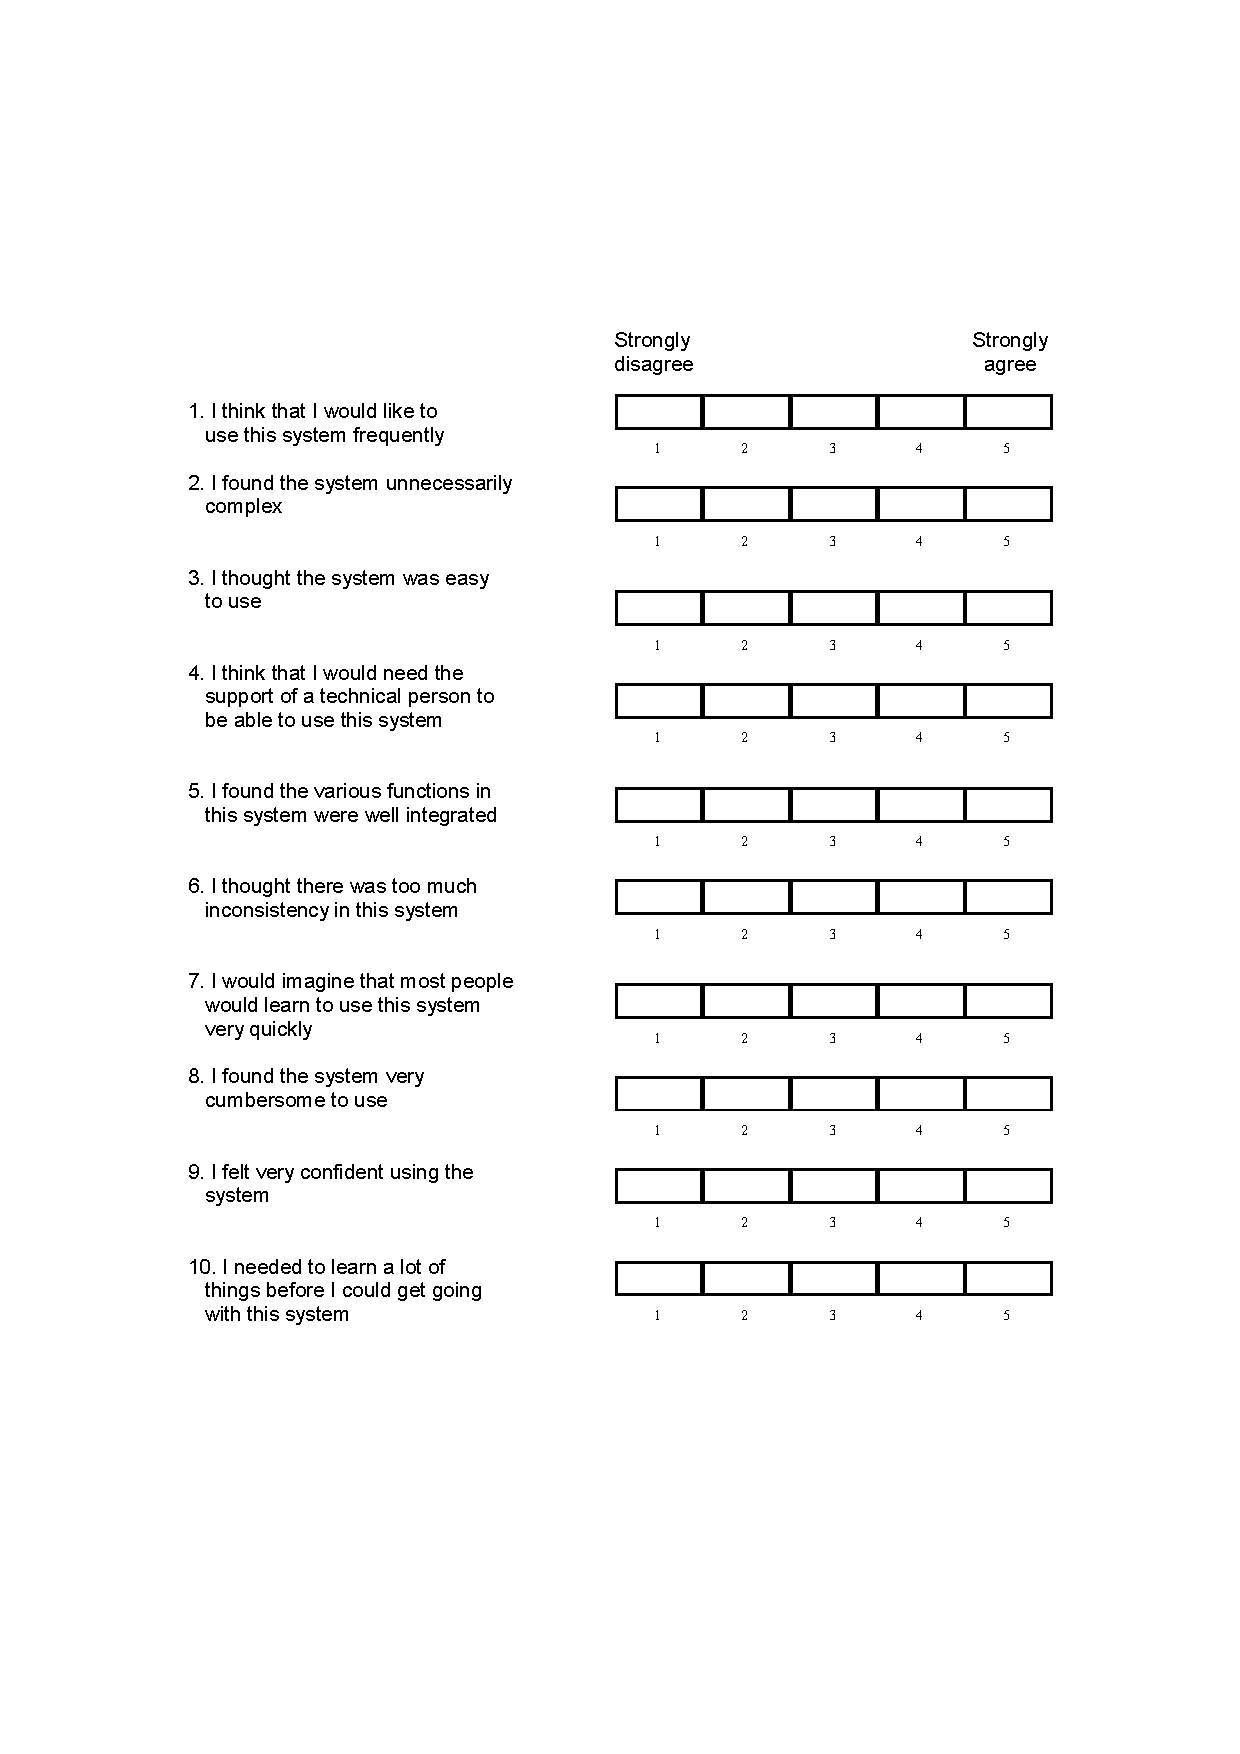
\includegraphics[width=1.0\textwidth]{./images/SUS.pdf}
    \caption{The \acf{SUS} Questionnaire}
    \label{fig:sus}
\end{figure}


%==============================================================================================================================================
\chapter{R Script for Plotting Data}
\label{app:r_script}

\section{Plotting Usage Adherence Data}

The following matrix shown the raw adherence scores used in the example shown in Table~\ref{tab:usage} and plotted in Figure~\ref{fig:usage}.

%\begin{figure}[h]
\begin{verbatim}
#  Month P1 P2 P3 P4 P5 P6 P7 P8 P9 P10 Total
1      3 28 NA NA NA NA NA NA NA NA  NA    28
2      4 30 14 NA NA NA NA NA NA NA  NA    44
3      5 29 21 18 28 NA NA NA NA NA  NA    96
4      6 25 22 13 29 NA NA NA NA NA  NA    89
5      7 29 14  6 29 18 NA NA NA NA  NA    96
6      8 24 12  4 25 21 NA NA NA NA  NA    86
7      9 NA 11  2 20 22 23 NA NA 28  NA   106
8     10 NA 12  2 14 14 22 NA NA 30  NA    94
9     11 NA 11 NA NA 14 22 NA NA 29  15    91
10    12 NA NA NA NA 16 24 NA NA 27  20    87
11    13 NA NA NA NA NA NA NA 12 29  22    63
12    14 NA NA NA NA NA NA NA  8 25  24    57
13    15 NA NA NA NA NA NA NA NA 23  25    48
14    16 NA NA NA NA NA NA 12 NA NA  25    37
15    17 NA NA NA NA NA NA 11 NA NA  NA    11
\end{verbatim}
%\caption{The example adherence data used in the plot shown in Figure~\ref{fig:usage}}
%\label{fig:adherence_data}
%\end{figure}

\noindent The following R scrips is used to generate the plots in  Figure~\ref{fig:usage}.


\begin{lstlisting}[language=R]
# A simple example of plotting fitted curves for usage adherence pr. participant and in total
# Jakob E. Bardram, 2017

library(ggplot2)
library(xts)
library(zoo)

#loading adherence data
adherence <- read.csv("~/Dropbox/WRITINGS/2017.CACHET.User.Study.Methodology/method/adherence.csv", sep=";")
adh_data <- adherence

# stacking the data into three columns [Month, Adherence, Participant] which is to be used by ggplot next
# note that the first and last columns of the adherence data are not included (Month and Total)
col_count <- ncol(adh_data) - 1
adh_frame <- data.frame(adh_data["Month"],stack(data.frame(coredata(adh_data[c(2:col_count)]))))
names(adh_frame) <- c("Month", "Adherence", "Participant")

# creating a theme for the graphs
t <-   theme(panel.background=element_rect(fill = "white"),
             panel.grid.minor = element_blank(),
             panel.grid.major = element_blank(),
             axis.line = element_line(colour = "black", size = 0.3),
             legend.background=element_rect(fill = "white"),
             legend.key=element_rect(fill = "white"),
             title = element_text(lineheight=.8, face="bold")
)

# plotting the data for all participants - showing both points and a smooth 'spline' trend line 
plot <- ggplot(adh_frame, aes(x=Month, y=Adherence, color=Participant))
plot <- plot + geom_point(aes(x=Month, y=Adherence, color=Participant), size = 1)
plot <- plot + geom_smooth(method = "lm", formula = y ~ splines::bs(x, 4), se = FALSE)
plot <- plot + ggtitle("Usage Adherence over time")
plot <- plot + t
plot

#stacking the Total column
adh_total <- data.frame(adh_data["Month"],data.frame(adh_data["Total"]))

#plotting the Total adherence over time, smooth
plot2 <- ggplot(adh_total, aes(x=Month, y=Total))
plot2 <- plot2 + geom_point(aes(x=Month, y=Total), size = 1)
plot2 <- plot2 + geom_smooth(method = "lm", formula = y ~ splines::bs(x, 7), se = FALSE)
plot2 <- plot2 + ggtitle("Usage Adherence over time, Total")
plot2 <- plot2 + t
plot2

# a plot of the data as a stacked area chart -- not smoothing, so not so nice...
plot3 <- ggplot(adh_frame, aes(x=Month, y=Adherence, color=Participant))
plot3 <- plot3 + 
  geom_area(aes(colour = Participant, fill= Participant), position = 'stack')
plot3 <- plot3 + 
  theme(panel.background=element_rect(fill = "white"),
        panel.grid.minor = element_blank(),
        panel.grid.major = element_blank(),
        axis.line = element_line(colour = "black", size = 0.3),
        legend.background=element_rect(fill = "white"),
        legend.key=element_rect(fill = "white"),
        plot.title = element_text(lineheight=.8, face="bold")
  )

plot3

\end{lstlisting}

\section{Generating Diverging Stacked Bar Charts for Likert Scale Data}

The R script generating the so-called `Diverging Stacked Bar Charts' for Likert scales visualization was originally proposed by Heiberger \& Robbins~\cite{heiberger2014design}). The following R script is used to generate Figure~\ref{fig:chart} from the data in Table~\ref{tab:survey} (without the `Total' and `Avg.' columns). The script is adopted from a script proposed by ´Wesley' at r-bloggers.com\footnote{https://www.r-bloggers.com/plotting-likert-scales/}.

\begin{lstlisting}[language=R]
# A simple example of a 'Diverging Stacked Bar Chart' for Likert Scale data on perceived usefulness and usability 
# Based on example from https://www.r-bloggers.com/plotting-likert-scales/
# Jakob E. Bardram, 2017

require(grid)
require(lattice)
require(latticeExtra)
require(HH)

#loading survey data
sgbar.likert<- survey
title<-"Perceived Usefulness and Usability of MySugar"

# A very simple plot -- out of the box
plot.likert(sgbar.likert, main=title)

# Changing the color palette
pal<-brewer.pal((numlevels-1),"RdBu")
pal[ceiling(numlevels/2)]<-"#DFDFDF"
# A slightly more tailored plot
plot.likert(sgbar.likert,
            main=title,
            col=pal,
            reference.line.col=c('black'),
            strip.left=FALSE,
            rightAxis=TRUE,
            sub="5-point Likert Scale"
)

\end{lstlisting}

